

\chapter{Corda Vibrante}

\section{Introduzione}

Obiettivo di questo esperimento è lo studio della propagazione di onde elastiche su una corda sotto l'azione di una forzante con andamento sinusoidale. Verifichiamo la dipendenza della frequenza dell'onda stazionaria in funzione della lunghezza, della massa lineare, della corda e dalla tensione applicata su di essa. 

\section{Strumenti}

\section{Ricerca delle armoniche}

Nella prima parte dell'esperienza, dopo aver trovato la frequenza di risonanza, abbiamo misurato le frequenze relative alle prime cinque armoniche di una corda vibrante di lunghezza $=111 cm$ e peso $5.21 g$ posta sotto una tensione $T$. La lunghezza $l$ è la distanza tra i punti di sospensione della corda: il primo coincidente nel punto di applicazione della forzante, il secondo è il punto di tangenza della carrucola.  
\\

Abbiamo ripetuto la misurazione sottoponendo la corda a quattro differenti forze di tensione (ottenute appendendo un peso ad una delle estremità della corda, come illustrato in figura) e per due corde di masse lineari $\mu$ differenti. 
\\
Nel seguente grafico, mostriamo la relazione tra la frequenza $\nu$ e il numero di armonica $N$. La relazione è lineare ed è la seguente equazione:
$$ \nu_n = 16.1n + 0.31 $$ 
\\
con $A= 0.31$, $\sigma_A=  0.93$ e $B=16.1, \sigma_B = 0.28 $ ricavati con il metodo dei minimi quadrati. 

\begin{center}

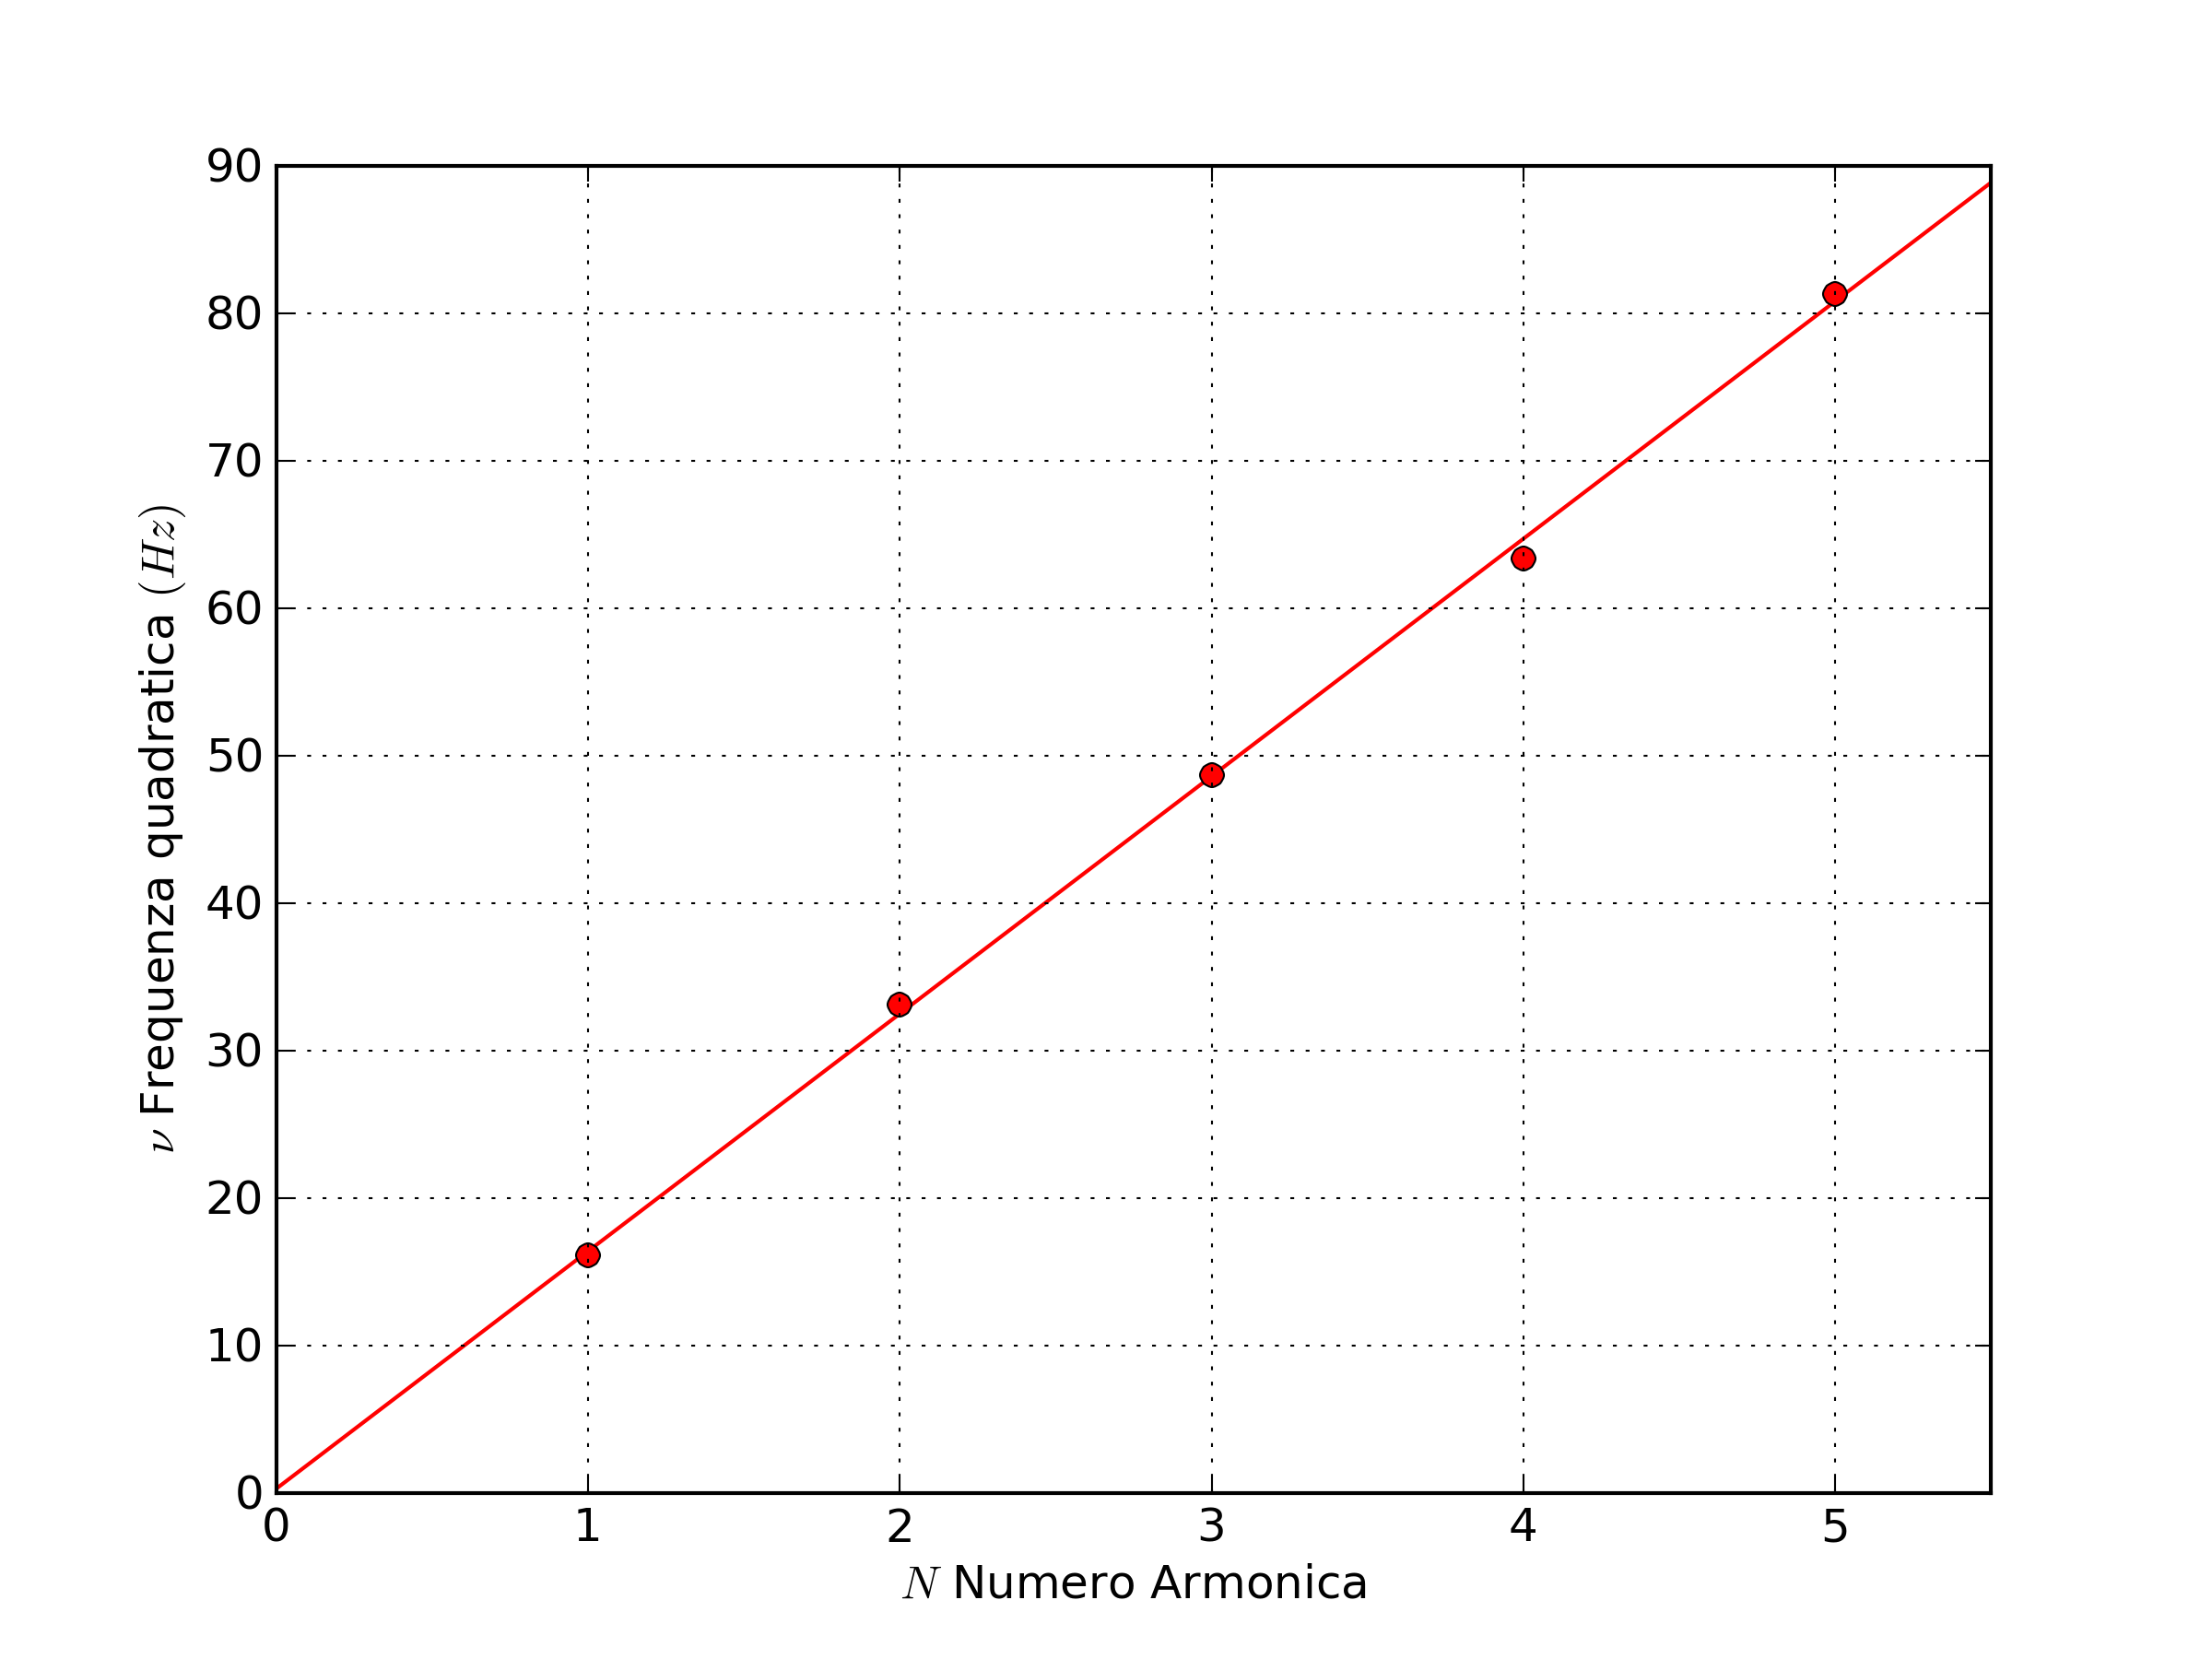
\includegraphics[scale=0.5]{../grafici/corda_1armonica}
\end{center}
Questo grafico è stato ricavato dalla corda A sottoposta ad una tensione $\tau=g\cdot250g$. Di seguito tutti i valori della frequenza di risonanza in funzione del numero di armonica e della tensione $\tau$ per valori crescenti della massa.

\begin{center}
\begin{tabular}{c   |  c}
\begin{tabular}{ c | c | c | c | c | c }
Massa($g$) & 1 & 2 & 3 & 4 & 5\\
\midrule
550 & 23.7 & 45.5 & 71.3 & 94.6 & 119.6\\
450 & 21,4 & 42,6 & 63,4 & 85,3 & 108,9\\
350 & 19.6 & 37.8 & 57.4 & 76.3 & 95.0\\
250 & 16.1 & 33.1 & 48.7 & 63.4 & 81.3 \\
\end{tabular}
&
\begin{tabular}{ c | c | c | c | c | c }
Massa($g$) & 1 & 2 & 3 & 4 & 5\\
\midrule
1050 & 19.3 & 38.4 & 56.1 & 75.2 & 94.7 \\
550 & 14.1 & 26.8 & 40.8 & 55.0 & 69.9 \\
450 & 13.1 & 25.4 & 38.9 & 51.7 & 64.2\\
350 & 10.9 & 22.8 & 35.2 & 46.9 & 58.3\\
\end{tabular}
\\
\end{tabular}
\end{center}
\section{Tensione e frequenza}
L'equazione $1$ mette in relazione la frequenza con la tensione. La relazione prevista è 

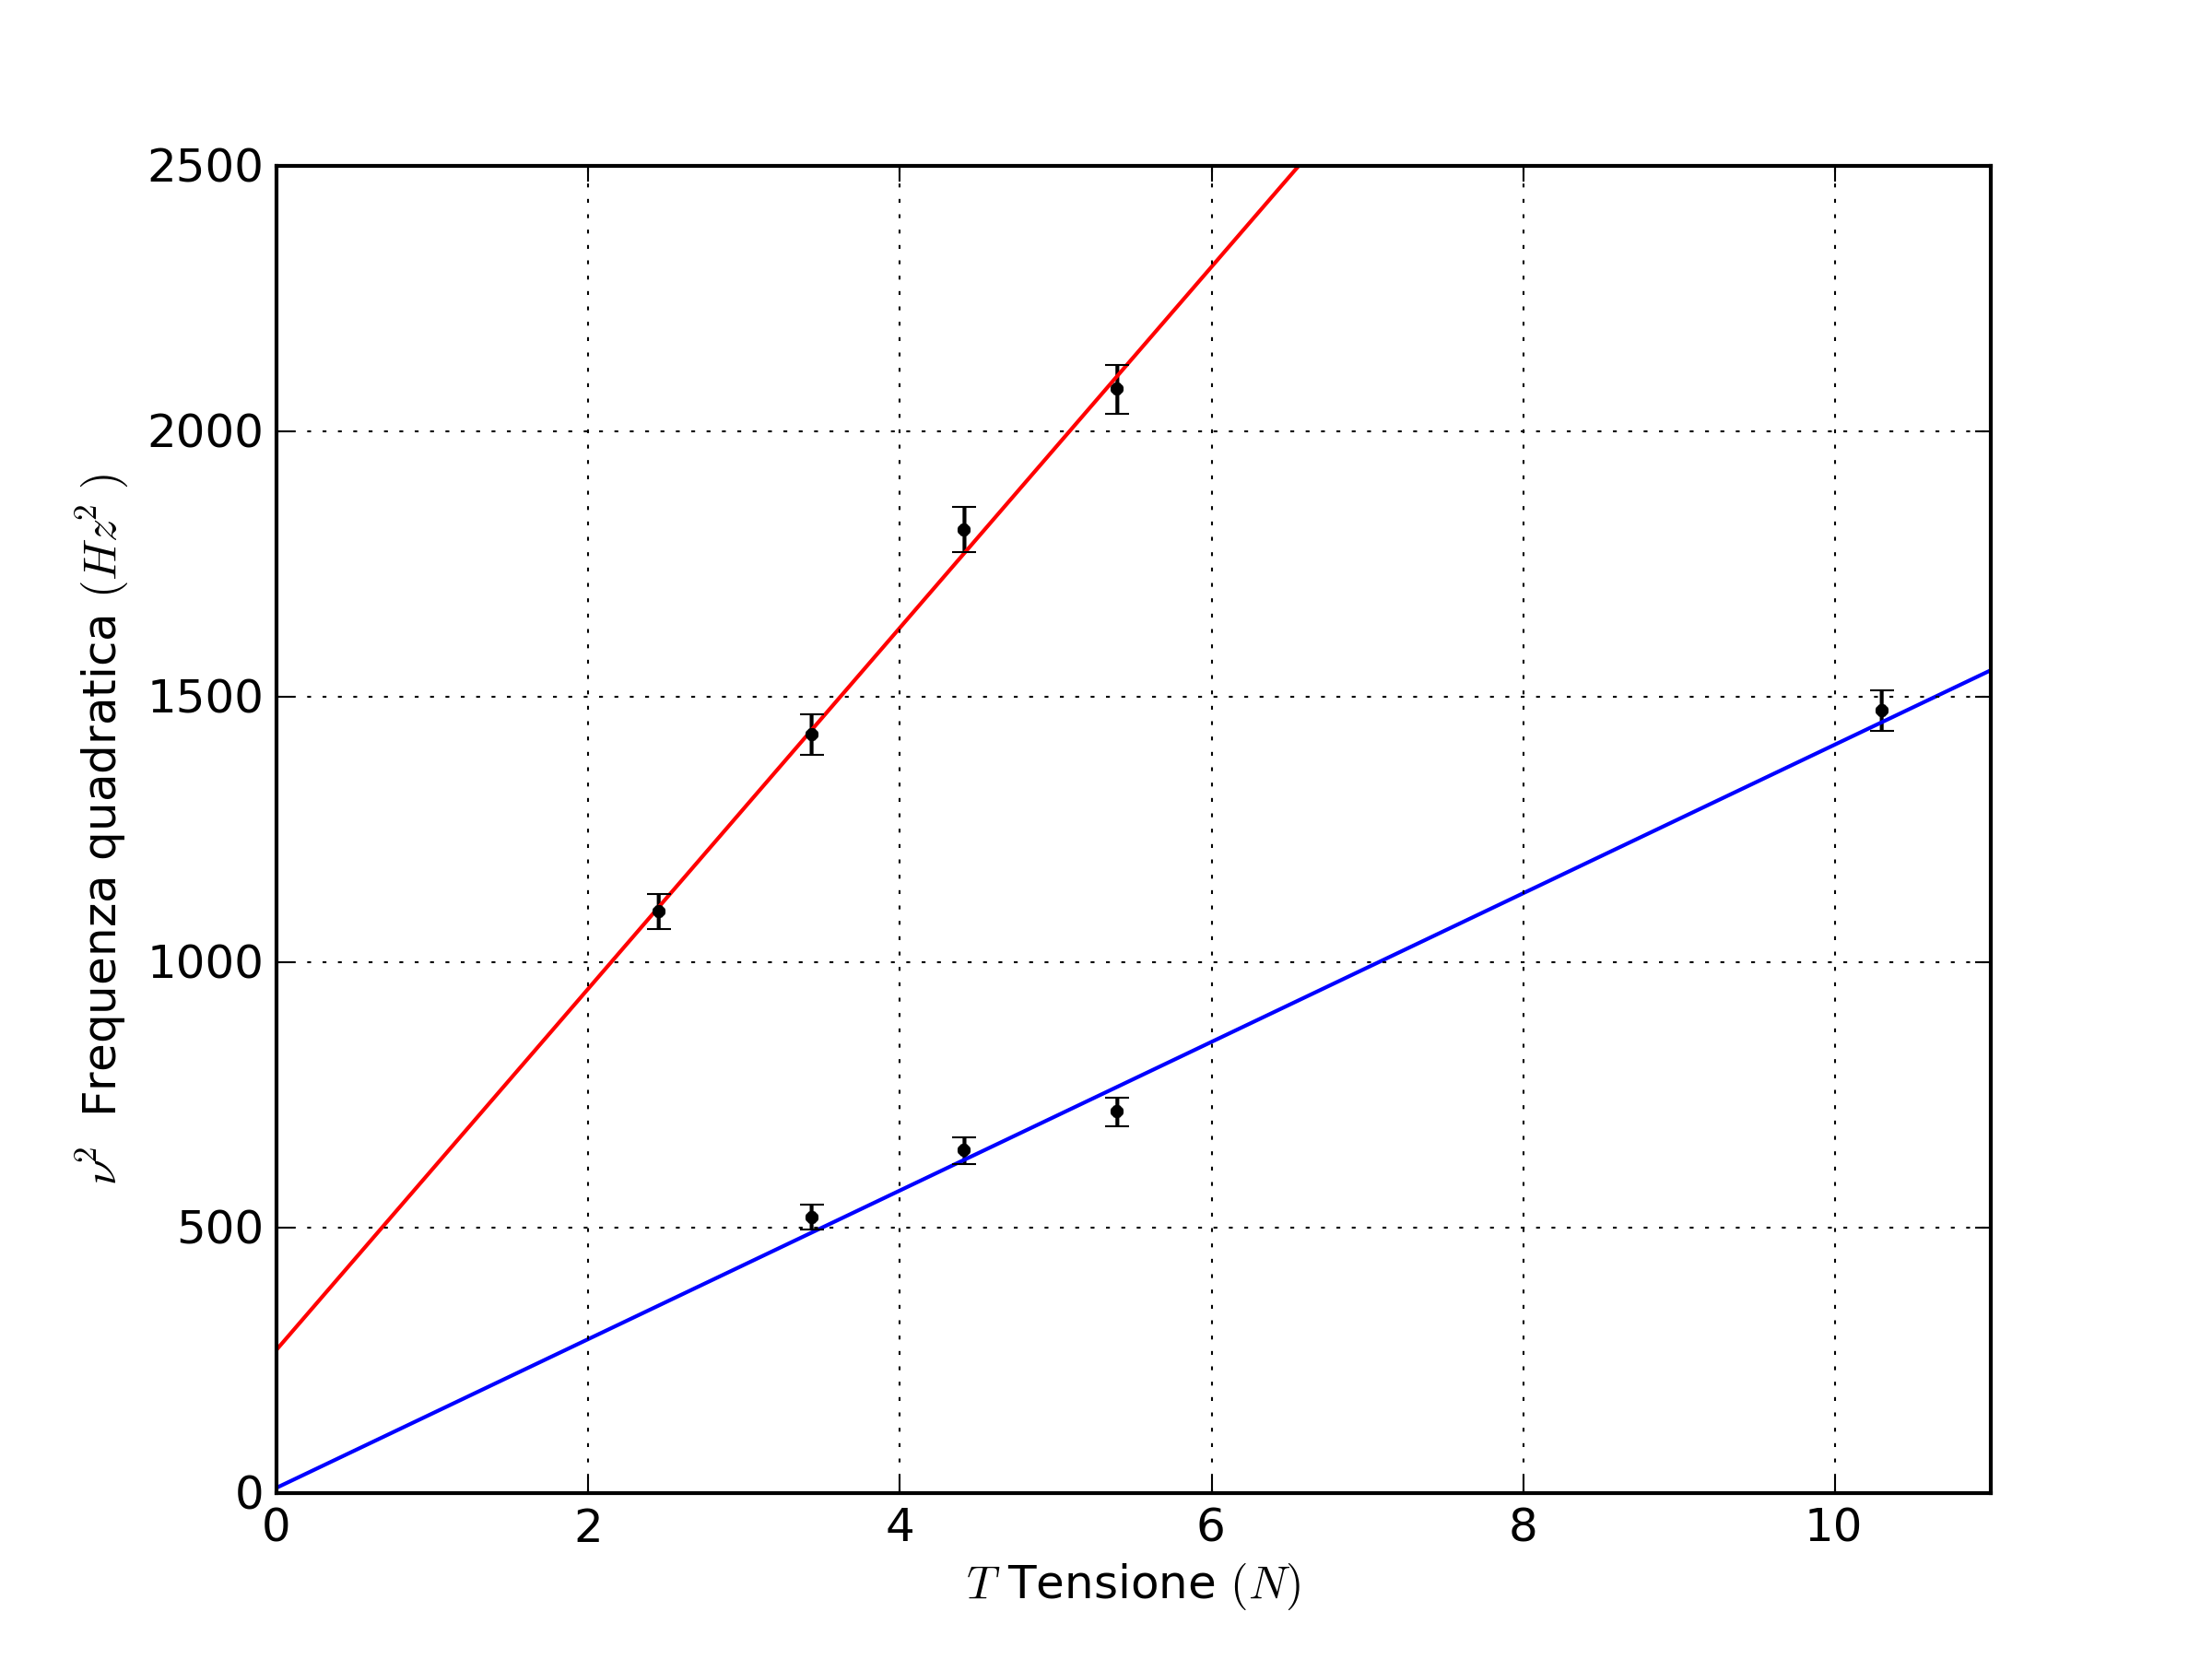
\includegraphics[scale=0.75]{../grafici/corda_tensione}


\begin{equation}
v=\sqrt{\frac{\tau}{\mu}}
\end{equation}

Le frequenze delle armoniche di ordine superiore sono date dall'equazione:
\begin{equation}
\nu=\frac{n}{2L}\sqrt{\frac{\tau}{\pi\rho}}
\end{equation}

dove L è la distanza tra i due punti di sospensione, $n\in \mathbb{N}$ è il numero dell'armonica, $\rho$ la densità della corda e $\tau$ la tensione.


\section{Dipendenza tra frequenza e lunghezza}

Velocità di propagazione di un'onda elastica in un mezzo materiale:
\begin{center}


\begin{tabular}{c|c}
L($cm$) & $\nu (Hz) $ \\
\midrule
105 & 24.6\\
111 & 23.7\\
116.5 & 22.8 \\
122.5 & 20.9 \\
131.5 & 20.1 \\
\end{tabular}
\end{center}

In tabella sono riportati i dati della frequenza delle prima armonica:

\begin{center}
\begin{tabular}{|c|c|}
\toprule
Lunghezza (m) & Frequenza (Hz) \\
\midrule
1.10 & 19.33 \\
1.15 & 18.25 \\
1.17 & 17.75 \\
1.22 & 17.00 \\
1.34 & 15.69 \\
1.53 & 13.92 \\
1.60 & 12.96 \\
0.91 & 22.83 \\
0.75 & 27.85 \\
0.60 & 35.00 \\
0.50 & 42.67 \\
\bottomrule
\end{tabular}
\end{center}

Inserendo questi dati su di un grafico, e interpolando la curva con Sage, troviamo il seguente grafico.

\includegraphics[scale=0.75]{"../grafici/CordaPrimaArmonica"}

Nota: $\rho$ è lasciato parametro libero, mentre invece $\tau$ è pari a 10.3 N, dato da un peso di 1.050 Kg sospeso a un'estremità della corda.

\section{Dipendenza tra frequenza e massa lineare}
